\section{Anal\'yza}

\subsection{Anal\'yza protokolu IPFIX}

Protokol IPFIX - \emph{IP Flow Information Export} je IETF \emph{(Internet Engineering Task Force)}
štandard pre export informácií o sieťových tokoch zo smerovačov, meracích sond, 
alebo špecializovaných nástrojov. 
Aby bolo možné prenášať tieto informácie 
od exportovacieho procesu k zhromažďovaciemu procesu, je potrebný štandardizovaný 
spôsob komunikácie a taktiež jednotná reprezentácia odovzdávaných dát.
Protokol je vyvíjaný rovnomennou pracovnou skupinou \citep{ipfixCharter} od roku 2001 a 
vznikol ako priamy nasledovník proprietárneho protokolu Cisco Netflow Version 9 \citep{rfc3954}. 
To znamená, že IPFIX je založený na systéme výmeny informácií na základe šablón. To ho robí veľmi
flexibilným, pretože je možné nakonfigurovať, ktoré vlastnosti tokov sa majú merať.
Zjednodušená architektúra protokolu IPFIX je na obrázku \ref{o:ipfix_architekture_basic}. 
\citep{rfc5101, ipfixProtocol, juvhaugen, veri}

\begin{figure}[ht!]
\centering
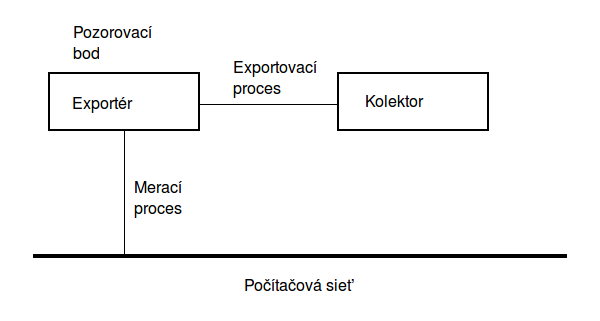
\includegraphics[width=0.7\textwidth]{ipfix_architekture_basic}
\caption{Zjednodušená verzia IPFIX architektúry}\label{o:ipfix_architekture_basic}
\end{figure}

\subsubsection{Terminológia} \label{sec:ipfix_terminology}

Podľa \citep{rfc3917} existuje veľa definícií termínu \uv{tok} používaných Internetovou komunitou.
Pracovná skupina IPFIX používa nasledujúcu:
\begin{description}
  \item[Tok] je definovaný ako množina IP paketov prechádzajúcich pozorovacím bodom v sieti, počas určitého 
časového intervalu. Všetky pakety patriace príslušnému toku majú množinu spoločných vlastností. Opačne, 
môžeme tvrdiť, že každý paket patrí toku, ak splna všetky tieto spoločné vlastnosti. 
\end{description}

Ďalšie termíny zavádza \citep{rfc5101}:
\begin{description}
  \item[Záznam o toku] obsahuje namerané informácie a charakteristické vlastnosti 
konkrétneho toku, ktorý bol pozorovaný pozorovacím bodom (napr. celkový počet prenesených 
bytov, zdrojová IP adresa toku, a pod.).

  \item[Pozorovací bod] je miestom v sieti, kde sú IP pakety pozorované. Medzi príklady patrí 
sieťová linka, na ktorej je zavedená meracia sonda, zdieľané médium (napr. Ethernet LAN), 
alebo fyzické, či logické rozhranie smerovača. Každý pozorovací bod je asociovaný s 
pozorovacou doménou. 

  \item[Pozorovacia doména] je množina pozorovacích bodov. Je identifikovaná číslom 
(Observation Domain ID), ktoré je unikátne v rámci exportovacieho procesu. 

  \item[Merací proces] vytvára záznamy o tokoch na základe hlavičiek paketov. Vykonáva 
rôzne funkcie ako napríklad odchytávanie hlavičiek paketov, vytváranie časových známok, 
vzorkovanie, klasifikovanie a údržba záznamov o tokoch. 

  \item[Exportovací proces] odosiela záznamy o tokoch zhromažďovacím 
procesom. Tieto záznamy sú generované jedným alebo viacerými meracími procesmi.
	
  \item[Exportér] odosiela dáta o tokoch. Je to nástroj ktorý zastrešuje exportovacie procesy.

  \item[Kolektor] je nástroj, ktorý prijíma dáta od exportéra. Pozostáva z jedného, alebo
viacerých zhromažďovacích procesov.

  \item[Zhromažďovací proces] prijíma záznamy o tokoch od jedného, alebo viacerých 
exportovacích procesov. Prijaté záznamy môže spracovávať, alebo uchovávať. 

  \item[Šablóna] špecifikuje formát odosielaných záznamov o tokoch pomocou zoznamu 
informačných elementov. Musí byť odoslaná kolektoru 
z exportovacieho procesu ešte pred odoslaním samotných dát. Neskor sú šablóny periodicky 
preposielané, aby kolektor vedel v každom okamihu aký formát dát prijme. 
Šablóny musia byť dostupné administrátorom, preto sú definované v konfiguračnom súbore 
exportéra.
\citep{juvhaugen}

% ---- tabulka ----
\tabcolsep=8pt
\begin{table}[!ht]\caption{Základné skupiny informačných elementov podla \citep{rfc5102}}\label{t:ie-table}
\smallskip
\centering
\begin{tabular}{|c|c|}
\hline
\textbf{\#} & \textbf{názov skupiny} \\ \hline
1. & Identifikátory \\ \hline
2. & Konfigurátory meracieho a exportovacieho procesu \\ \hline
3. & Štatistické hodnoty meracieho a exportovacieho procesu \\ \hline
4. & Polia IP hlavičky \\ \hline
5. & Polia transportnej hlavičky \\ \hline
6. & Polia ostatných hlavičiek \\ \hline
7. & Odvodené vlastnosti paketov \\ \hline
8. & Min/Max vlastnosti tokov \\ \hline
9. & Časové známky tokov \\ \hline
10. & Počítadla vlastností tokov \\ \hline
11. & Rôzne vlastnosti tokov \\ \hline
12. & Padding \\ \hline
\end{tabular}
\end{table}
% -----------

  \item[Informačné elementy] sú protokolovo nezávislým popisom atribútov záznamov o tokoch. 
Informačný model IPFIX \citep{rfc5102} obsahuje základnú množinu informačných elementov, vrátane ich
popisu, významu, dátového typu a pod. Informačné elementy sú rozdelené do 12 skupín, pozri tabuľku \ref{t:ie-table},
na základe ich sémantiky a použitia. Každý element je asociovaný s dátovým typom, ktorý určuje jeho 
formát a spôsob kódovania.
Na základe tohto modelu sú jednotlivé dátové záznamy kódované na strane exportéra a dekódované 
v kolektore.\\
Informačný model povoľuje aj jeho rozširovanie. Organizácie môžu definovať vlastné informačné
elementy, ktorým musia prideliť unikátny identifikátor. 
Tieto elementy navyše obsahujú identifikátor organizácie (PEN), ktorý musí byť registrovaný v IANA
\footnote{http://www.iana.org/assignments/enterprise-numbers}.
\end{description}

\subsubsection{Formát IPFIX správ} \label{sec:message_format}

Formát správ je definovaný v Špecifikácii IPFIX Protokolu \citep{rfc5101}. Správa pozostáva z 
hlavičky, nasledovaná niekoľkými IPFIX sadami. 
Exportér musí zakódovať všetky časti správy v sieťovom poradí bytov (Big-Endian).
Na obrázku \ref{o:ipfix_message_format} je jedna z možností formátu IPFIX správy. Za hlavičkou nasleduje sada šablón, pretože
šablóny musia byť exportované ihneď po vytvorení. Za šablónami nasledujú dátové sady a sady šablón možností 
v akomkoľvek poradí.

\begin{figure}[ht!]
\centering
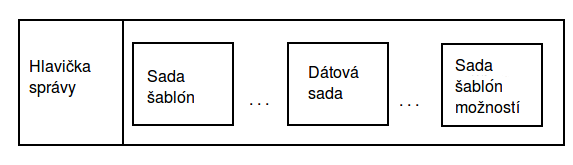
\includegraphics[width=0.7\textwidth]{ipfix_message_format}
\caption{Príklad formátu IPFIX správy}\label{o:ipfix_message_format}
\end{figure}

\paragraph{Formát hlavičky správy}

Formát hlavičky správy je znázornený na obrázku \ref{o:ipfix_message_header}. Pozostáva z piatich poli:
\begin{itemize}
 \item \textbf{Číslo verzie} záznamu toku v správe. Pre IPFIX je to hodnota \verb|0x000a|.
 \item \textbf{Dĺžka} predstavuje celkovú dĺžku IPFIX správy v oktetoch, vrátane hlavičky a sád. 
 \item \textbf{Čas exportu} vo formáte UNIX timestamp. 
 \item \textbf{Sekvenčné číslo} vyjadruje počet odoslaných záznamov dátových záznamov modulo $2^{32}$  
 exportovacím procesom v tejto transportnej relácii. Túto hodnotu používa kolektor na odhalenie chýbajúcich 
 správ resp. dátových šablón.
 \item \textbf{Identifikačné číslo pozorovacej domény}, ktorý je lokálne jedinečný pre exportovací proces.
 \end{itemize}
 
\begin{figure}[ht!]
\centering
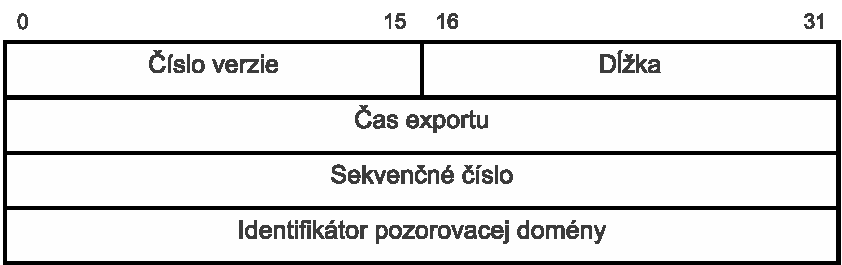
\includegraphics[width=0.7\textwidth]{ipfix_message_header}
\caption{Formát hlavičky IPFIX správy}\label{o:ipfix_message_header}
\end{figure}

\paragraph{Formát sady}

V IPFIX terminológii je sada všeobecný pojem pre kolekciu záznamov s podobnou štruktúrou. 
IPFIX správa môže obsahovať tri rôzne druhy sád:
\begin{itemize}
 \item Sada šablón
 \item Dátová sada
 \item Sada šablón možností
\end{itemize}
Každá zo sad sa skladá z hlavičky sady a jedného, alebo viacerých záznamov sady, obrázok \ref{o:set_format}. 
Na úplnom konci môže byt vložený padding, no nie je to povinná súčasť sady. Exportovací proces ho pridáva 
iba v tom prípade, keď chce aby sada bola zarovnaná na dĺžku, ktorá je násobkom 4, alebo 8.

\begin{figure}[ht!]
\centering
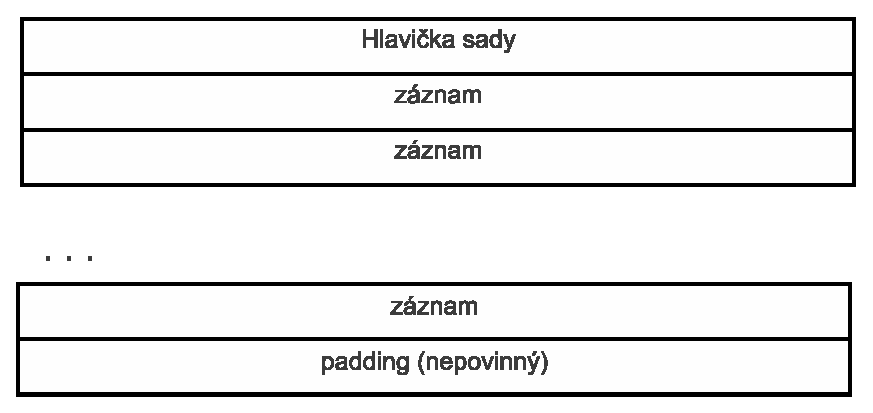
\includegraphics[width=0.7\textwidth]{set_format}
\caption{Formát sady}\label{o:set_format}
\end{figure}

\textbf{Hlavička sady} je rovnaká pre všetky tri typy sád. Je zobrazená na obrázku \ref{o:set_header}. 
\emph{Identifikátor sady} určuje typ sady a teda aj typ všetkých záznamov obsiahnutých v sade, pozri 
\ref{t:set-record}. 
Sada istého druhu nemôže obsahovať záznamy iného typu. 
Hodnotu 2 je rezervovaná pre sadu šablón. Sada šablón možností nadobúda 
hodnotu 3. Identifikátory 0 a 1 sa nepoužívajú z historických dôvodov \citep{rfc3954} a hodnoty od 4 po 
255 sú rezervované pre budúce použitie. Dátové sady sú označené hodnotami väčšími ako 255. 

% ---- tabuľka ----
\tabcolsep=8pt
\begin{table}[!ht]\caption{Prehľad identifikátorov, typov a záznamov sady}\label{t:set-record}
\smallskip
\centering
\begin{tabular}{|c|c|c|}
\hline
\textbf{Identifikátor sady} & \textbf{typ sady} & \textbf{typ záznamov} \\ \hline
0 - 1 & -- & -- \\ \hline
2 & sada šablón & záznamy šablóny \\ \hline
3 & sada šablón možností & záznamy šablóny možností \\ \hline
4 - 255 & -- & -- \\ \hline
255 - 65535 & dátová sada & dátové záznamy \\ \hline
\end{tabular}
\end{table}
% -----------

\emph{Dĺžka sady} zahŕňa celková dĺžka všetkých sád, vrátane hlavičky sady a prípadne paddingu. Na jej základe 
sa určuje začiatok ďalšej sady, pretože sada môže obsahovať rôzny počet záznamov.

\begin{figure}[ht!]
\centering
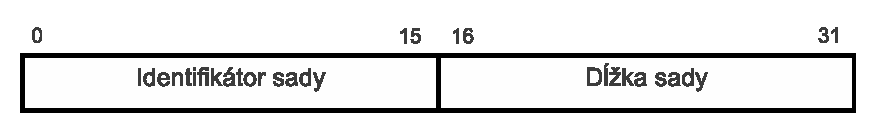
\includegraphics[width=0.7\textwidth]{set_header}
\caption{Formát hlavičky sady}\label{o:set_header}
\end{figure}

\paragraph{Špecifikátory poľa}

Špecifikátor poľa je akousi obálkou nad informačným elementom, obrázok \ref{o:field_specifier_format}, 
vďaka nemu vie zhromažďovací proces spracovávať prijaté dáta. 

Prvý bit sa nazýva \emph{Enterprise bit}.
Ak je nastavený na 0, tak hovoríme o oficiálnom informačnom elemente charakterizovanom organizáciou IETF a 
registrovanom v IANA. 
V tomto prípade je \emph{číslo organizácie (PEN)} nevyplnené. V opačnom prípade, 
keď je tento bit nastavený na 1, ide o organizáciou špecifikovaný informačný element a číslo organizácie
musí byť zadané. Laboratórium Počítačových Sietí na Technickej Univerzite v Košiciach má pridelené číslo 
organizácie 26235 \citep{pen}.
Dĺžka poľa vyjadruje na koľkých oktetoch je daný informačný element kódovaný. 
Zoznam informačných elementov aj s ich dĺžkami je dostupný v \citep{rfc5102}.
Špeciálny prípad nastáva pri redukovanom kódovaní. Vtedy je dĺžka poľa menšia ako popisuje 
Informačný model. 
 
\begin{figure}[ht!]
\centering
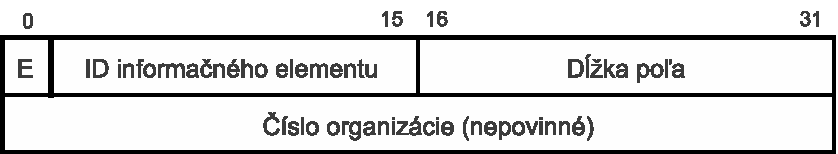
\includegraphics[width=0.7\textwidth]{field_specifier_format}
\caption{Formát špecifikátora poľa}\label{o:field_specifier_format}
\end{figure}



\paragraph{Formát záznamov šablóny}

Záznamy šablóny patria k nevyhnutným prvkom IPFIX správy. Na ich základe, a základe Informačného modelu
IPFIX \citep{rfc5102} vie zhromažďovací proces dekódovať dátové záznamy.
Šablóny môžu obsahovať akúkoľvek kombináciu informačných elementov. Či už oficiálnych, navrhnutých 
spoločnosťou IANA, alebo vlastných, vytvorených organizáciami.

Záznam šablóny tvorí \emph{hlavička}, pozri \ref{o:template_record_header}, nasledovaná 
\emph{špecifikátormi poľa}. 
Každá šablóna musí mať v rámci transportnej relácie a pozorovacej domény jedinečný \emph{identifikátor}. 
Čísluje sa od 255 do 65535, rovnako ako identifikátory dátových sád, pretože každá šablóna referuje 
na dátovú sadu, ktorej štruktúru popisuje. \emph{Počet polí} sa týka počtu 
špecifikátorov poľa.

\begin{figure}[ht!]
\centering
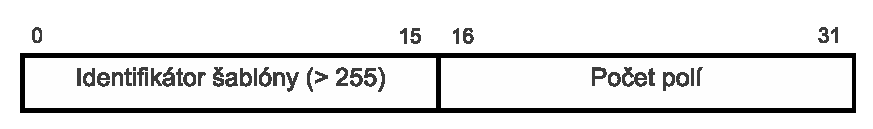
\includegraphics[width=0.7\textwidth]{template_record_header}
\caption{Formát hlavičky záznamu šablóny}\label{o:template_record_header}
\end{figure}

\paragraph{Formát záznamov šablóny možností}

Tieto záznamy dávajú exportéru možnosť poskytnúť kolektoru dodatočné informácie o kontexte posielaných dát, 
ktoré by zo samotných 
záznamov tokov nevedel vyčítať. Príkladom týchto informácií sú kľúče tokov, alebo konfigurácia šablóny,
vzorkovacie parametre a pod.

Formát záznamov \ref{o:options_record_header} je podobný ako v prípade záznamov šablóny. Pozostáva z hlavičky záznamu 
a jedného, alebo viacerých špecifikátorov poľa. Formát špecifikátorov je rovnaký ako pri záznamoch šablóny.
Hlavička naviac obsahuje \emph{počet polí pôsobnosti}. Pôsobnosť charakterizuje kontext 
informácií. Šablóna povoľuje 
definovať viac polí pôsobnosti ako jedno. V tomto prípade je celková pôsobnosť daná kombináciou týchto polí.
Počet polí pôsobnosti nemôže byť nulový, pričom \emph{počet polí} je 
súčtom polí pôsobnosti a špecifikátorov poľa.

\begin{figure}[ht!]
\centering
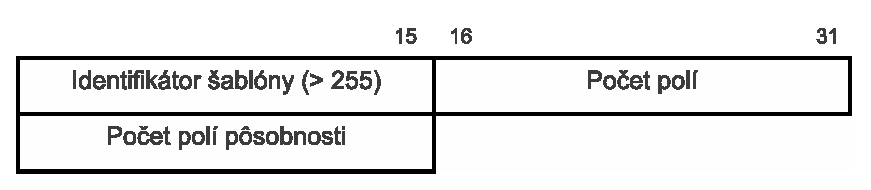
\includegraphics[width=0.7\textwidth]{options_record_header}
\caption{Formát hlavičky záznamu šablóny možností}\label{o:options_record_header}
\end{figure}

\paragraph{Formát dátových záznamov}

Dátové záznamy sú posielané v dátových sadách. Ich formát je veľmi 
jednoduchý. Pozostávajú len z hodnôt polí, nemajú ani vlastnú hlavičku. 
Sú kódované podla popisu v Informačnom modeli \citep{rfc5102}. Identifikátor 
šablóny, ktorá popisuje tieto hodnoty je zakódovaný v hlavičke sady, v časti
identifikátor sady. Inými slovami \uv{identifikátor sady} = \uv{identifikátor 
šablóny}. Aby vedel kolektor tieto dáta dekódovať, musí poznať formát šablóny 
už pred prijatím prvého dátového záznamu.
